\chapter{La complejidad algorítmica}
\label{chap:notacion-asintotica}

Cuando tenemos que resolver un problema, es posible que estén disponibles varios algoritmos adecuados. Evidentemente, desearíamos seleccionar el mejor. Esto plantea la pregunta de cómo decidir entre varios algoritmos cuál es preferible. Si solamente tenemos que resolver uno o dos casos pequeños de un problema más bien sencillo, quizá no nos importe demasiado qué algoritmo utilizaremos: en este caso podríamos decidirnos a seleccionar sencillamente el que sea más fácil de programar, o uno para el cual ya exista un programa, sin preocuparnos por sus propiedades teóricas. Sin embargo, si tenemos que resolver muchos casos, o si el problema es difícil, quizá tengamos que seleccionar de forma más cuidadosa.\\

El enfoque \emph{empírico} (o a posteriori) para seleccionar un algoritmo consiste en programar las técnicas competidoras e ir probándolas en distintos casos con ayuda de una computadora. El enfoque \emph{teórico} (a priori) que es el que casi siempre se toma como referencia, consiste en determinar matemáticamente la cantidad de recursos necesarios para cada uno de los algoritmos \emph{como función del tamaño de los casos considerados}. Los recursos que más nos interesan son el tiempo de computación y el espacio de almacenamiento, siendo el primero normalmente el más importante. \\

El \emph{tamaño} de un ejemplar se corresponde formalmente con el número de \emph{bits} que se necesitan para representar el ejemplar en una computadora, utilizando algún esquema de codificación precisamente definido y razonablemente compacto. Sin embargo, para hacer más claros nuestros análisis, lo normal será que seamos menos formales, y utilizaremos la palabra ``tamaño'' para indicar cualquier entero que mida de alguna forma el número de componentes de un ejemplar. Por ejemplo, cuando estamos hablando acerca de ordenaciones, mediremos normalmente el tamaño de un ejemplar por el número de items que hay que ordenar ignorando el hecho consistente en que cada uno de estos items ocuparía más de un bit para representarlo en una computadora. De manera similar, cuando hablemos acerca de grafos, mediremos normalmente el tamaño de un ejemplar por el número de nodos o de aristas (o de ambos) implicados. Apartándonos un poco de esta regla general, sin embargo, cuando hablemos acerca de problemas que impliquen enteros, daremos algunas veces la eficiencia de nuestros algoritmos en términos del \emph{valor} del ejemplar que estemos considerando, en lugar de considerar su tamaño (que sería el número de \emph{bits} necesarios para representar en binario este valor).\\

La ventaja de la aproximación teórica es que no depende ni de la computadora que se esté utilizando, ni del lenguaje de programación, ni siquiera de las habilidades del programador. Se ahorra tanto el tiempo que se habría invertido innecesariamente para programar un algoritmo ineficiente, como el tiempo de máquina que se habría desperdiciado comprobándolo. Lo que es más significativo, se nos permite estudiar la eficiencia del algoritmo cuando se utiliza en casos de todos los tamaños. Esto no suele suceder con la aproximación empírica, en la cual las consideraciones prácticas podrían obligarnos a comprobar los algoritmos sólo en un pequeño número de ejemplares arbitrariamente seleccionados y de tamaño moderado. Dado que suele suceder que los algoritmos recién descubiertos empiezan a comportarse mejor que sus predecesores sólo cuando ambos se utilizan en ejemplares grandes, este último punto resulta especialmente importante. \\

Si deseamos medir la cantidad de espacio que utiliza un algoritmo en función del tamaño de los ejemplares, está a nuestra disposición una unidad natural, a saber, el \emph{bit}. Independientemente de la máquina que se esté utilizando, la noción de un \emph{bit} de almacenamiento está bien definida. Si, por otra parte, tal como suele suceder, deseamos medir la eficiencia de un algoritmo, en términos del tiempo que se necesita para llegar a una respuesta, entonces no existe una opción tan evidente. Está claro que no se puede pensar en expresar esta eficiencia, digamos, en segundos, puesto que no se dispone de una computadora estándar a la cual se pudieran referir todas las medidas (existe una computadora estándar, pero es un modelo teórico: la maquina de Turing).\\

Una respuesta a este problema es la que viene dada por el \emph{principio de invariancia}, que afirma que dos implementaciones distintas de un mismo algoritmo no diferirán en su eficiencia en más de alguna constante multiplicativa. Si esta constante fuera, por ejemplo, cinco, entonces sabemos que si la primera implementación requiere un segundo para resolver casos de un cierto tamaño, entonces la segunda implementación (quizá en una máquina distinta, o escrita en un lenguaje de programación distinto) no requerirá más de 5 segundos para resolver los mismos casos. Para ser más exactos, si dos implementaciones del mismo algoritmo necesitan $t_1(n)$ y $t_2(n)$ segundos, respectivamente, para resolver un caso de tamaño $n$, entonces siempre existen constantes positivas $c$ y $d$ tales que $t_1(n) \leq ct_2(n)$ y $t_2(n) \leq dt_1(n)$ siempre que $n$ sea lo suficientemente grande. En otras palabras, el tiempo de ejecución de cualquiera de las implementaciones está acotado por un múltiplo constante del tiempo de ejecución de la otra; la decisión de a qué implementación llamaremos primera, y a cuál llamaremos segunda, es irrelevante. La condición de que $n$ sea suficientemente grande no es realmente necesaria, según la \textbf{regla del umbral}:\\

\begin{fondo}
Una función $t_n$ pertenece al orden de $f(n):\ O(f(n))$
\begin{itemize}
\item cuando está acotada superiormente por $f(n)$ para valores de $n$ suficientemente grandes y
\item haciendo abstracción de posibles constantes multiplicativas
\end{itemize}
\begin{center}
\[O(f(n)) = \Bigl\{ t: \mathbb{N} \rightarrow \mathbb{R}^{\geq 0} \Bigl| \exists\ c \in \mathbb{R}^{+} , \exists n_{0} \in \mathbb{N} \Bigl| \forall n \geq n_{0} : t(n) \leq c \cdot f(n) \Bigl\} \]
\end{center}

\end{fondo}

Sin embargo, al incluirla suele ser posible hallar constantes más pequeñas $c$ y $d$ que las que se hallarían en caso contrario. Esto resulta útil si estamos intentando calcular buenas cotas acerca del tiempo de ejecución de una implementación cuando conocemos el tiempo de ejecución de la otra.\\

Volviendo a la cuestión de la unidad que se debe utilizar para expresar la eficiencia teórica de un algoritmo, el principio de invariancia nos permite decidir que no va a existir tal unidad. En su lugar, expresaremos solamente el tiempo requerido por el algoritmo salvo una constante multiplicativa. Diremos que un algoritmo para algún problema requiere un tiempo del orden de $t(n)$ para una función dada $t$, si existe una constante positiva $c$ y una implementación del algoritmo capaz de resolver todos los casos de tamaño $n$ en un tiempo que no sea superior a $ct(n)$ segundos. \\

El uso de segundos en esta definición es evidentemente arbitrario: sólo se necesita modificar la constante para acotar el tiempo por $at(n)$ años o por $bt(n)$ microsegundos. Por el principio de invariancia, si cualquier implementación del algoritmo tiene la propiedad requerida, entonces también la tienen todas las demás, aunque la constante multiplicativa pueda cambiar de una implementación a otra.\\

\section{Notación asintótica}

Esta notación se denomina ``asintótica'' porque trata acerca del comportamiento de funciones en el límite, esto es, para valores suficientemente grandes de su parámetro. En consecuencia, los argumentos basados en la notación asintótica pueden no llegar a tener un valor práctico cuando el parámetro adopta valores ``de la vida real''. Sin embargo, en las enseñanzas de la notación asintótica suelen tener una relevancia significativa. Esto se debe a que, un algoritmo que sea superior asintóticamente suele ser (aunque no siempre) preferible incluso en casos de tamaño moderado.\\

\subsection{La $O$ mayúscula}

Sea $t: \mathbb{N} \rightarrow \mathbb{R}^{\geq 0}$ una función arbitraria de los números naturales en los números reales no negativos, tal como $t(n) = 5n^2 + \frac{100}{3}n + 2$. Se suele pensar que $n$ representa el tamaño del ejemplar sobre el cual es preciso que se aplique un algoritmo dado, y en $t(n)$ como representante de la cantidad de un recurso dado que se invierte en ese ejemplar por una implementación particular de este algoritmo. Por ejemplo, podría ser que la implementación invirtiera $t(n)$ microsegundos en el ejemplar peor en un caso de tamaño $n$, o quizá $t(n)$ represente la cantidad de espacio. Tal como se ha visto, la función $t(n)$ puede muy bien depender de la implementación más que depender únicamente del algoritmo. Recuerde sin embargo el principio de invariancia, que dice que la \emph{razón} de los tiempos de ejecución de dos implementaciones diferentes del mismo algoritmo siempre está acotada por encima y por debajo mediante constantes predeterminadas. (Las constantes pueden depender de las implementaciones pero no del tamaño del ejemplar).\\

Considérese ahora una función $f: \mathbb{N} \rightarrow \mathbb{R}^{\geq 0}$ tal como $f(n) = n^2$. Diremos que $t(n)$ está en el \emph{orden de f(n)} si $t(n)$ está acotada superiormente por un múltiplo real positivo de $f(n)$ para todo $n$ suficientemente grande. Matemáticamente, esto significa que existe una constante real y positiva $c$ y un entero umbral $n_0$ tal que $t(n) \leq cf(n)$, siempre que $n \geq n_0$.\\

Por ejemplo, considérese las funciones $f(n)$ y $t(n)$ definidas anteriormente. Está claro que tanto $n \leq n^2$ como $1 \leq n^2$, siempre que $n \geq 1$. Por tanto, siempre y cuando $n \geq 1$:

\begin{center}
\[ t(n) = 5n^2 + \frac{100}{3}n + 2 \]
\[ \geq 5n^2 + \frac{100}{3}n^2 + 2n^2 \]
\[ = 40n^2 = 40 f(n) \]
\end{center}

Tomando $c = 40$ (o cualquier valor mayor) y $n_0 = 1$, concluiremos por tanto que $t(n)$ es del orden de $f(n)$ por cuanto $t(n) \leq cf(n)$ siempre que $n \geq n_0$. Por tanto es conveniente disponer de un símbolo matemático para representar \emph{el orden de}. Una vez más sea $f: \mathbb{N} \rightarrow \mathbb{R}^{\geq 0}$ una función arbitraria de los números naturales en los reales no negativos. Le indicará mediante $O(f(n))$ - que se lee ``$O$ de $f(n)$'' - \emph{el conjunto} de todas las funciones $t: \mathbb{N} \rightarrow \mathbb{R}^{\geq 0}$ tales que $t(n) \leq cf(n)$ para todo $n \geq n_0$ para una constante positiva real $c$ y para un umbral entero $n_0$. En otras palabras:
\begin{center}
\[ O(f(n)) = \big\{ t: \mathbb{N} \rightarrow \mathbb{R}^{\geq 0} \big| \exists c \in \mathbb{R}^+\ \exists n_0 \in \mathbb{N}\ \forall n \geq n_0\ [t(n) \leq cf(n)] \big\} \]\\
\end{center}

\begin{nota}
A partir de ahora la notación del término $O(f(n))$ será $O(f)$ empleada en otros libros o referencias para facilitar su uso al lector. Igualmente la notación para la función $f(n)$ se sustituirá con la notación simple de $f$ siempre que no haya confusión.\\
\end{nota}

La notación $O(f)$, denota al conjunto de las funciones de $t$ que crecen a lo más tan rápido como $f$, es decir, las funciones $t$ tales que, mediante una \emph{constante multiplicativa}, $f$ llega a ser en algún momento una cota superior para $t$. Así pues la correspondencia con la definición es intuitiva: el cuantificador existencial sobre $c$ formaliza la expresión \emph{constantes multiplicativas}, y $n_0$ indica a partir de qué punto $f$ es realmente una cota superior para $t$.\\

A modo de ejemplo, aplicando la definición puede comprobarse que para $f(n) = n^2$ y $t(n) = n$ se tiene que $t \in O(f))$ pero sin embargo $f \notin O(t)$. Para $f(n) = 3n^2$ y $t(n) = 100n^2$ se tiene que $t \in O(f)$ y $f \in O(t)$.\\

La notación $O(f)$ tiene las siguientes propiedades, cualesquiera que sean las funciones $f,t$ y $g$.\\
\begin{enumerate}
\item \emph{Invariancia multiplicativa}. Para toda constante $c \in \mathbb{R}^+$,
\[ t \in O(f) \iff c \cdot t \in O(f) \]
Se demuestra por simple aplicación de la definición.
\item \emph{Reflexividad}. $f \in O(f)$. Basta comprobar la definición.
\item \emph{Transitividad}. Si $g \in O(t)$ y $t \in O(f)$ entonces $g \in O(f)$. Se demuestra mediante sencillas manipulaciones aritméticas.
\item \emph{Criterio de caracterización}. $t \in O(f) \iff O(t) \subseteq O(f)$. Se deduce fácilmente de las dos anteriores.
\item \emph{Regla de la suma para $O$}. $O(f+t) = O(max(f,t))$, donde denotamos $f+t$ la función que sobre el argumento $n$ vale $f(n)+t(n)$, y $max(f,t)$ la función sobre la que el argumento $n$ vale el máximo de $\{f(n),t(n)\}$. Frecuentemente esta regla se aplica así: si $t_1 \in O(f_1)$ y $t_2 \in O(f_2)$, entonces $t_1 + t_2 \in O(max(f_1,f_2))$.
\item \emph{Regla del producto para $O$}. Si $t_1 \in O(f_1)$ y $t_2 \in O(f_2)$, entonces $t_1 \cdot t_2 \in O(f_1 \cdot f_2)$, donde denotamos $f \cdot t$ la función que sobre el argumento $n$ vale $f(n) \cdot t(n)$.
\item \emph{Invariancia aditiva}. Para toda constante $c \in \mathbb{R}^{+}$,
\[ t \in O(f) \iff c + t \in O(f) \]
En consecuencia inmediata de la regla de la suma.
\end{enumerate}

\subsection{Formas de crecimiento frecuentes}

La escala a la cual clasificaremos el uso de recursos de los algoritmos consiste en una serie de funciones elegidas entre las que es posible definir por operaciones aritméticas, logaritmos y exponenciales. A lo largo de esta sección, y salvo indicación explícita de lo contrario, la base de todos los logaritmos es 2 (si bien en la mayoría de los casos la independencia de factores constantes da lugar a que la base del algoritmo sea indiferente).\\
Las más importantes formas de crecimiento asintótico son las siguientes:\\
\begin{itemize}
\item Constante: $O(1)$. El coste de aplicación de un algoritmo con complejidad constante puede ser acotado independientemente de la talla del problema.
\[ O(1) = O(c), \forall c \in \mathbb{R}^+, c > 0 \]
\item Logarítmico: $O(\log n)$
\item Lineal: $O(n)$
\item Quasilineal: $O(n \cdot \log n)$
\item Cuadrático: $O(n^2)$
\item Cúbico: $O(n^3)$
\item Polinómico: $O(n^k)$ con $k$ fijo.
\item Exponencial: $O(k^n)$ con $k > 1$ y fijo.
\item Complejidad $n!$: $O(n!)$
\end{itemize}

La jerarquía de órdenes de complejidad es importante comentarla más profundamente.\\
La siguiente figura muestra el aspecto de las funciones representativas de dichos órdenes. A simple vista no se aprecian quizás las implicaciones prácticas de dicha figura. Para ilustrar mejor las diferencias, supongamos que tenemos diferentes algoritmos para un problema dado con tiempos tales que su menor cota superior en el peor caso está respectivamente en los órdenes $O(\log n)$, $O(n)$, $O(n \cdot \log n)$, $O(n^2)$, $O(n^3)$ y $O(2^n)$.\\

Supongamos que para un tamaño del problema $n = 100$, todos ellos tardarán un tiempo $t = 1$ hora en ejecutarse con un ordenador y lenguaje determinados. Estudiaremos dos casos diferentes: por un lado, estudiaremos el tiempo necesario para resolver un problema de un tamaño dado y de un tamaño dos y diez veces mayor (n=100, n=200 y n=1000); por otro lado duplicaremos y multiplicaremos por 10 el tiempo disponible ($t=1$ hora, $t=2$ horas y $t=10$ horas) (sería equivalente a mantener el tiempo y duplicar y multiplicar por 10 la velocidad del ordenador) y calcularemos el tamaño del mayor problema que es posible tratar en dicho tiempo con cada algoritmo.\\

\begin{center}%
\begin{figure}[H]%
\begin{minipage}[H]{1\columnwidth}%
\centering%
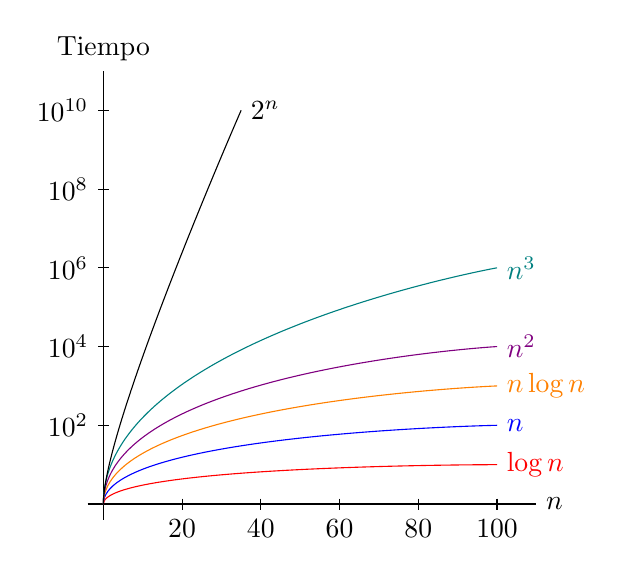
\begin{tikzpicture}

  \draw[] (-0.2,0) -- (5.5,0) node[right] {$n$};
  \draw[] (0,-0.2) -- (0,5.5) node[above] {Tiempo};

  \foreach \x/\xtext in {1/20, 2/40, 3/60, 4/80, 5/100}
  \draw[shift={(\x,0)}] (0pt,2pt) -- (0pt,-2pt) node[below] {$\xtext$};

  \foreach \y/\ytext in {1/10^2, 2/10^4, 3/10^6, 4/10^8, 5/10^{10}}
  \draw[shift={(0,\y)}] (2pt,0pt) -- (-2pt,0pt) node[left] {$\ytext$};

  \draw[red] (0,0)   .. controls +(up:.5cm) and +(left:0cm) .. (5,.5) node [right] {$\log n$};
  \draw[blue] (0,0)   .. controls +(up:.9cm) and +(left:0cm) .. (5,1) node [right] {$n$};
  \draw[orange] (0,0)   .. controls +(up:1.3cm) and +(left:0cm) .. (5,1.5) node [right] {$n \log n$};
  \draw[violet] (0,0)   .. controls +(up:1.7cm) and +(left:0cm) .. (5,2) node [right] {$n^2$};
  \draw[teal] (0,0)   .. controls +(up:2.1cm) and +(left:0cm) .. (5,3) node [right] {$n^3$};
  \draw[] (0,0)   .. controls +(up:1cm) and +(left:0cm) .. (1.75,5) node [right] {$2^n$};

\end{tikzpicture}
\caption{Representación gráfica de las tasas de crecimiento más frecuentes.}%
\end{minipage}%
\end{figure}%
\end{center}%

\vspace*{-.5in}{
El resultado queda reflejado en las siguientes tablas:
\begin{table}[H]
\begin{center}
\begin{tabular}{|c|c|c|c|}
\hline
$t(n)$ & $n=100$ & $n=200$ & $n=1000$ \\
\hline
$k_1\ \log n$ & $1$ h. & $1,15$ h. & $1,5$ h. \\
\hline
$k_2 n$ & $1$ h. & $2$ h. & $10$ h. \\
\hline
$k_3\ n \log n$ & $1$ h. & $2,30$ h. & $15$ h. \\
\hline
$k_4 n^2$ & $1$ h. & $4$ h. & $100$ h. \\
\hline
$k_5 n^3$ & $1$ h. & $8$ h. & $1000$ h. \\
\hline
$k_6 2^n$ & $1$ h. & $1,27\ \cdot\ 10^{30}$ h. & $8,45\ \cdot\ 10^{270}$ h. \\
\hline
\end{tabular}
\caption{Efecto de duplicar y multiplicar por diez el tamaño del problema.}
\end{center}
\end{table}

\begin{table}[H]
\begin{center}
\begin{tabular}{|c|c|c|c|}
\hline
$t(n)$ & Tiempo=1h. & Tiempo=2h. & Tiempo=10h. \\
\hline
$k_1\ \log n$ & $n=100$  & $n=10.000$ & $n=10^{20}$ \\
\hline
$k_2 n$ & $n=100$  & $n=200$ & $n=1000$ \\
\hline
$k_3\ n \log n$ & $n=100$ & $n=178$ & $n=703$ \\
\hline
$k_4 n^2$ & $n=100$ & $n=141$ & $n=316$ \\
\hline
$k_5 n^3$ & $n=100$ & $n=126$ & $n=215$ \\
\hline
$k_6 2^n$ & $n=100$ & $n=101$ & $n=103$ \\
\hline
\end{tabular}
\caption{Efecto de duplicar y multiplicar por diez el tamaño del problema.}
\end{center}
\end{table}}

Los que se comportan de un modo más acorde con las expectativas de un usuario no informático son los de complejidad \emph{lineal} y $O(n \log n)$: al duplicar y multiplicar por diez el tamaño del problema aproximadamente se duplica y se multiplica por diez el tiempo empleado, y al duplicar y multiplicar por diez el tiempo disponible, el tamaño que es posible tratar también se duplica y multiplica por diez.\\

El algoritmo de complejidad \emph{logarítmica} tiene un comportamiento excepcionalmente bueno: doblar y multiplicar por diez el tamaño del problema solo aumenta moderadamente el tiempo de ejecución ($15\%$ y $50\%$, respectivamente), mientras que doblar y multiplicar por diez el tiempo disponible permite tratar problemas enormes ($100$ y $10^{18}$ veces mayores que el problema original).\\

Los órdenes $O(n^2)$ y $O(n^3)$ tienen un comportamiento claramente inferior al lineal. Se observa que un incremento del $100\%$ en el tiempo disponible sólo consigue incrementos respectivamente del $41\%$ y del $26\%$ en el tamaño del problema, incluso al multiplicar por 10 el tiempo disponible solo permite resolver problemas 3,16 y 2,15 veces mayores respectivamente. En general podemos decir que dado un algoritmo de orden $O(n^a)$, multiplicar el tiempo disponible (o la velocidad del computador) por un factor $k$ multiplica el tamaño del problema que es posible tratar por un factor $\varphi^k$. Estos cálculos llevan a la conclusión de que no es posible tratar problemas demasiado grandes con algoritmos que presenten estas tasas de crecimiento.\\

No obstante, los algoritmos cuyas tasas de crecimiento están acotadas superiormente por $n^a$ (para cualquier $a$) se dicen, en conjunto, de complejidad polinomial, y los problemas que resuelven se llaman \textbf{tratables}.\\

La situación es muy distinta para los problemas de complejidad exponencial o mayor, que se llaman \textbf{intratables}. Se llaman así los problemas cuyos mejores algoritmos conocidos tiene tiempos en $O(2^n)$. Un algoritmo de tiempo de ejecución exponencial permite tratar problemas muy pequeños, independientemente de la velocidad del ordenador; observando las tablas vemos que multiplicar el tiempo apenas afecta al tamaño del problema que podemos resolver, y multiplicar el tamaño del problema conduce, en este ejemplo, a tiempos de ejecución del orden de varios billones (como mínimo) de veces la edad del universo.\\

Estas consideraciones nos llevan a la conclusión de que es una buena inversión dedicar tiempo a encontrar algoritmos con mejores tasas de crecimiento. Por ejemplo, pasar un algoritmo de $O(n^2)$ a otro de $O(n \log n)$ es una gran mejora, y lo mismo podríamos decir si se encontrara un algoritmo de $O(\log n)$ para problemas que se resolvían en $O(n)$.\\

En sentido contrario, invertir tiempo en ahorrar ésta o aquella variable en un programa, o en mejorar algún caso particular, no cambia generalmente la tasa de crecimiento del algoritmo, sino tan sólo disminuye ligeramente la constante multiplicativa. Además suele oscurecer su comprensión, por tanto no es una inversión rentable e incluso puede llegar a ser contraproducente. \\

\subsection{Indecibilidad}
\label{sec:indecibilidad}

El propósito de esta sección es proporcionar una introducción informal, basada en el lenguaje de programación C, para mostrar un problema específico que los computadores no pueden resolver. El problema concreto que vamos a examinar tiene por objeto detectar si lo primero que imprime un programa C es \emph{hola, mundo}. Aunque podría imaginarse que la simulación del programa nos permitiría descubrir lo que hace, en realidad tenemos que enfrentarnos con programas que tardan un tiempo inimaginable largo para producir alguna respuesta. Este problema (no saber cuándo ocurre algo, si es que llega ha producirse) es la causa última de nuestra incapacidad para descubrir lo que hace un programa. Sin embargo, es bastante difícil demostrar formalmente que no existe ningún programa capaz de realizar una cierta tarea preestablecida, y es necesario desarrollar algún mecanismo para ello. \\

\newpage

\subsubsection{Programas que imprimen ``hola, mundo''}

En el siguiente fragmento de código se presenta el primer programa en C que encuentran los estudiantes que leen el ya clásico libro de Kernighan y Ritchie\footnote{B.W. Kernighan y D.M. Ritchie, \emph{The C Programming Language}, 1978, Prentice-Hall, Englewood Cliffs, NJ.}. Es bastante fácil descubrir que este programa imprime \emph{hola, mundo} y termina. El programa es tan simple que se ha convertido en una práctica habitual introducir los lenguajes de programación cómo se escribe un programa que imprima \emph{hola, mundo} en dichos lenguajes. \\

\begin{Verbatim}[commandchars=\\\{\}]
\PY{c+cp}{\PYZsh{}}\PY{c+cp}{include<stdio.h>}

\PY{k+kt}{int} \PY{n+nf}{main}\PY{p}{(}\PY{p}{)}
\PY{p}{\PYZob{}}
  \PY{n}{printf}\PY{p}{(}\PY{l+s}{"}\PY{l+s}{hola, mundo}\PY{l+s+se}{\PYZbs{}n}\PY{l+s}{"}\PY{p}{)}\PY{p}{;}

  \PY{k}{return} \PY{l+m+mi}{0}\PY{p}{;}
\PY{p}{\PYZcb{}}
\end{Verbatim}


Sin embargo, existen otros programas que también imprimen \emph{hola, mundo} a pesar de que lo que hacen no es ni mucho menos evidente. El siguiente fragmento de código presenta otro programa que quizá imprima \emph{hola, mundo}. Este programa toma una entrada $n$ y busca soluciones enteras positivas de la ecuación $x^n + y^n = z^n$. Si encuentra una solución, imprime \emph{hola, mundo}. Si nunca encuentra enteros $x, y$ y $z$ que satisfagan la ecuación, entonces continúa buscando para siempre, y nunca imprime \emph{hola, mundo}.\\

Para comprender qué hace el programa, digamos primero que $exp$ es una función auxiliar para calcular potencias. El programa principal tiene que buscar las tuplas $(x,y,z)$ en un orden tal que estemos seguros de encontrar, finalmente, todas las tuplas de enteros positivos. Para organizar la búsqueda de forma apropiada, se utiliza una cuarta variable, \emph{total}, cuyo valor inicial es 3, y que, en el bucle while, va incrementándose en una unidad, tomando siempre valores enteros finitos. Dentro del bucle while, \emph{total} se divide en tres números enteros positivos, $x, y,$ y $z$, haciendo primero que $x$ varíe desde 1 hasta \emph{total-2}, y, dentro del bucle for, haciendo que $y$ varíe desde 1 hasta una unidad menos de lo que queda de \emph{total} después de haberle restado el valor actual de $x$. A $z$ se le asigna la cantidad restante, que debe estar entre 1 y \emph{total-2}.\\

\underline{El último teorema de Fermat expresado como un programa hola-mundo}
\begin{Verbatim}[commandchars=\\\{\}]
\PY{c+cp}{\PYZsh{}}\PY{c+cp}{include <stdlib.h>}
\PY{c+cp}{\PYZsh{}}\PY{c+cp}{include <stdio.h>}

\PY{k+kt}{int} \PY{n+nf}{exp}\PY{p}{(}\PY{k+kt}{int} \PY{n}{i}\PY{p}{,} \PY{k+kt}{int} \PY{n}{n}\PY{p}{)}
\PY{c+cm}{/* calcula i a la potencia n */}
\PY{p}{\PYZob{}}
  \PY{k+kt}{int} \PY{n}{ans}\PY{p}{,} \PY{n}{j}\PY{p}{;}
  \PY{n}{ans} \PY{o}{=} \PY{l+m+mi}{1}\PY{p}{;}
  \PY{k}{for} \PY{p}{(}\PY{n}{j}\PY{o}{=}\PY{l+m+mi}{1}\PY{p}{;} \PY{n}{j} \PY{o}{<}\PY{o}{=} \PY{n}{n}\PY{p}{;} \PY{n}{j}\PY{o}{+}\PY{o}{+}\PY{p}{)} \PY{n}{ans} \PY{o}{*}\PY{o}{=} \PY{n}{i}\PY{p}{;}
  \PY{k}{return}\PY{p}{(}\PY{n}{ans}\PY{p}{)}\PY{p}{;}
\PY{p}{\PYZcb{}}

\PY{k+kt}{int} \PY{n+nf}{main}\PY{p}{(}\PY{p}{)}
\PY{p}{\PYZob{}}
  \PY{k+kt}{int} \PY{n}{n}\PY{p}{,} \PY{n}{total}\PY{p}{,} \PY{n}{x}\PY{p}{,} \PY{n}{y}\PY{p}{,} \PY{n}{z}\PY{p}{;}
  \PY{n}{scanf}\PY{p}{(}\PY{l+s}{"}\PY{l+s}{\PYZpc{}d}\PY{l+s}{"}\PY{p}{,}\PY{o}{&}\PY{n}{n}\PY{p}{)}\PY{p}{;}
  \PY{n}{total} \PY{o}{=} \PY{l+m+mi}{3}\PY{p}{;}
  \PY{k}{while}\PY{p}{(}\PY{l+m+mi}{1}\PY{p}{)}\PY{p}{\PYZob{}}
    \PY{k}{for}\PY{p}{(}\PY{n}{x}\PY{o}{=}\PY{l+m+mi}{1}\PY{p}{;} \PY{n}{x} \PY{o}{<}\PY{o}{=} \PY{n}{total} \PY{o}{-} \PY{l+m+mi}{2}\PY{p}{;} \PY{n}{x}\PY{o}{+}\PY{o}{+}\PY{p}{)}
      \PY{k}{for}\PY{p}{(}\PY{n}{y}\PY{o}{=}\PY{l+m+mi}{1}\PY{p}{;} \PY{n}{y} \PY{o}{<}\PY{o}{=} \PY{n}{total} \PY{o}{-}\PY{n}{x} \PY{o}{-}\PY{l+m+mi}{1}\PY{p}{;} \PY{n}{y}\PY{o}{+}\PY{o}{+}\PY{p}{)}
	\PY{p}{\PYZob{}}
	  \PY{n}{z} \PY{o}{=} \PY{n}{total} \PY{o}{-} \PY{n}{x} \PY{o}{-} \PY{n}{y}\PY{p}{;}
	  \PY{k}{if}\PY{p}{(}\PY{n}{exp}\PY{p}{(}\PY{n}{x}\PY{p}{,}\PY{n}{n}\PY{p}{)} \PY{o}{+} \PY{n}{exp}\PY{p}{(}\PY{n}{y}\PY{p}{,}\PY{n}{n}\PY{p}{)} \PY{o}{=}\PY{o}{=} \PY{n}{exp}\PY{p}{(}\PY{n}{z}\PY{p}{,}\PY{n}{n}\PY{p}{)}\PY{p}{)}
	    \PY{n}{printf}\PY{p}{(}\PY{l+s}{"}\PY{l+s}{hola, mundo}\PY{l+s+se}{\PYZbs{}n}\PY{l+s}{"}\PY{p}{)}\PY{p}{;}
	\PY{p}{\PYZcb{}}
    \PY{n}{total}\PY{o}{+}\PY{o}{+}\PY{p}{;}
  \PY{p}{\PYZcb{}}
\PY{p}{\PYZcb{}}
\end{Verbatim}


En el bucle más interno, se comprueba si la tupla $(x,y,z)$ verifica la ecuación $x^n + y^n = z^n$. Si es así, el programa imprime \emph{hola, mundo}, y si no, no imprime nada.\\

Si el valor de $n$ leído por el programa es 2, entonces acabará encontrando combinaciones de enteros tales como $total = 12, x = 3, y = 4$ y $z = 5$, para las cuales $x^n + y^n = z^n$. De modo que, teniendo 2 como entrada, \emph{sí} imprime \emph{hola, mundo}.\\

Sin embargo, para cualquier entero $n > 2$, el programa nunca encontrará una tupla de enteros positivos que satisfaga $x^n + y^n = z^n$ y, por tanto, nunca llegará a imprimir \emph{hola, mundo}. Lo curioso del caso es que hasta hace pocos años no se sabía si este programa imprimiría o no \emph{hola, mundo} para algunos número enteros $n$ grandes. La afirmación de que no lo haría, esto es, de que no existen soluciones enteras para la ecuación $x^n y^n = z^n$ si $n > 2$, fue realizada por Fermat hace 300 años, pero no pudo demostrarse hasta hace bastante poco. Esta proposición recibe a menudo el nombre de ``último teorema de Fermat''.\\

Definamos así el \emph{problema hola-mundo}: determinar si un programa C dado, con una cierta entrada, imprime en primer lugar los 11 caracteres de \emph{hola, mundo}. \\

Parece probable que, si a los matemáticos les llevó 300 años resolver una pregunta acerca de un único programa de 22 líneas, entonces debe ser realmente difícil decidir el problema general de si un programa dado, con una cierta entrada, imprime o no \emph{hola, mundo}. De hecho, cualquiera de los problemas que los matemáticos todavía no han podido resolver puede plantearse como una pregunta de la forma ``¿este programa, con esta entrada, imprime \emph{hola, mundo}?''. Así que sería realmente extraordinario que fuéramos capaces de escribir un programa que pudiera examinar cualquier programa $P$ y cualquier entrada $I$ para $P$ y decir si $P$, al ejecutarlo con $I$ como entrada, imprimirá \emph{hola, mundo}. Dicha demostración de que tales programas no existen queda fuera de este contexto de estudio.\\

\subsubsection{Por qué tienen que existir problemas indecidibles}

Aunque es delicado demostrar que un problema específico, como el ``problema hola-mundo'' que acabamos de examinar, es indecidible, es bastante sencillo comprender por qué casi todos los problemas han de ser indecidibles para los sistemas relacionados con la programación. Recordemos que un ``problema'' en realidad se ha definido como una pregunta acerca de si cierta cadena forma parte de un lenguaje. El número de lenguajes diferentes con cualquier alfabeto de más de un símbolo no es numerable; esto es, no hay forma de asignar números enteros a los lenguajes de manera que cada lenguaje tenga asignado un número entero y cada número entero corresponda a un lenguaje. \\

Por otra parte, los programas \emph{son} numerables, por ser cadenas finitas construidas con un alfabeto finito (normalmente, un subconjunto del alfabeto ASCII). Es decir, es posible ordenarlos de acuerdo con su longitud, por orden alfabético. Por tanto, podemos hablar del primer programa, el segundo programa y, en general, del $i$-ésimo para cualquier entero $i$.\\

Como consecuencia, sabemos que existen infinitos programas menos que problemas. Si eligiéramos un lenguaje al azar, casi seguro que correspondería a un problema indecidible. La única razón por la que la mayoría de los problemas \emph{parece} que son decidibles es porque los problemas elegidos al azar rara vez tienen interés. Más bien, tendemos a considerar problemas bastante sencillos y bien estructurados, y estos problemas que nos interesan, y que pueden enunciarse clara y brevemente, es posible encontrar muchos indecidibles; el problema hola-mundo es uno de ellos.\\

\vspace{-.25in}{
\subsection{La máquina de Turing}

La teoría de los problemas indecidibles no solo tiene por objeto establecer la existencia de dichos problemas (una idea emocionante por sí sola desde el punto de vista intelectual), sino proporcionar a los programadores una guía sobre lo que se puede llevar a cabo o no llevar a cabo mediante la programación. Para los programadores y diseñadores de sistemas, estos problemas, llamados ``problemas intratables'', tienden a presentar más dificultades que los problemas indecidibles. La razón para ello es que, mientras que suele ser obvio que los problemas indecidibles efectivamente lo son y, en la práctica, raramente se intentan resolver, los problemas intratables aparecen continuamente. Además, a menudo dan lugar a pequeñas modificaciones de los requisitos o a soluciones heurísticas. Por tanto, los diseñadores tienen que enfrentarse frecuentemente al hecho de tener que decidir si un problema es o no intratable, y qué hacer si lo es.\\}

Hacen falta herramientas que nos permitan determinar la indecidibilidad  o intratabilidad de los problemas de cada día. La tecnología que se introdujo en la sección anterior es útil para las cuestiones que se plantean acerca de los programas, pero no se puede trasladar fácilmente a problemas de otros dominios no relacionados. Por ejemplo, podríamos tener grandes dificultades para reducir el problema hola-mundo a la cuestión de si una gramática es ambigua.\\

En consecuencia, necesitamos reconstruir la teoría de la indecibilidad, no ya basándonos en programas escritos en C o cualquier otro lenguaje de programación, sino en un modelo muy simple de computador, denominado máquina de Turing. Este dispositivo es esencialmente un autómata finito que dispone de una cinta de longitud infinita sobre la que puede leer y escribir datos. Una de las ventajas de la máquina de Turing sobre los programas, como mecanismo de representación de lo que se puede computar, es que la máquina de Turing es suficientemente sencilla como para que su configuración pueda representarse con precisión, utilizando una notación simple del estilo de las configuraciones de los autómatas a pila. En cambio, aunque los programas en C tiene un estado, que depende de todas las variables, sea cual sea la secuencia de llamadas a las función que se realice, la notación que hay que utilizar para describirlo es demasiado compleja como para permitirnos realizar demostraciones formales comprensibles.\\

Utilizando la notación de la máquina de Turing, probaremos que son indecidibles ciertos problemas que, aparentemente, no tienen relación con la programación.\\

\subsubsection{El intento de decidir todas las cuestiones matemáticas}

A finales del siglo XIX, el matemático D. Hilbert se preguntó si era posible encontrar un algoritmo para determinar la verdad o falsedad de cualquier posición matemática. En particular, se preguntaba si existiría un modo de determinar si cualquier fórmula del cálculo de predicados de primer orden, aplicada a enteros, es verdadera. Dado que el cálculo de predicados de primer orden sobre los enteros es suficientemente potente como para expresar frases como ``esta gramática es ambigua'', o ``este programa imprime \emph{hola, mundo}'', si Hilbert hubiera tenido éxito, existirían algoritmos para dichos problemas, que ahora sabemos que no existen.\\

Sin embargo, en 1931, K. Gödel publicó su famoso teorema de la incompletitud. Gödel construyó una fórmula del cálculo de predicados aplicado a enteros que afirmaba que la propia fórmula no podía ser probada, ni refutada, dentro del cálculo de predicados. \\

El cálculo de predicados no era la única idea que tenían los matemáticos para ``cualquier computación posible''. De hecho, el cálculo de predicados, al ser declarativo más que computacional, entraba en competencia con una variedad de notaciones, incluidas las ``funciones recursivas parciales'' (una notación parecida a un lenguaje de programación) y otras notaciones similares. En 1936, A.M. Turing propuso la máquina que lleva su nombre como modelo de ``cualquier computación posible''. Este modelo se parece más a un computador que a un programa, aunque los verdaderos computadores electrónicos, o incluso los electromecánicos, tardaron varios años en llegar. \\

Lo curioso del caso es que todas las propuestas serias sobre modelos de computación tienen el mismo potencial, es decir, computan exactamente las mismas funciones y reconocen los mismos lenguajes. La suposición no demostrada de que cualquier forma general de computación nos permitirá calcular únicamente las funciones recursivas parciales (o, lo que es lo mismo, lo que las máquinas de Turing o los computadores modernos pueden calcular) se conoce como \emph{hipótesis de Church}(en honor al lógico A. Church) o \emph{tesis de Church-Turing}.\\

\subsection{Notación para la máquina de Turing}

Podemos imaginarnos una máquina de Turing como la que se ha presentado en la siguiente figura. La máquina consta de una \emph{unidad de control}, que puede estar en cualquier estado tomado de un conjunto finito. Hay una cinta dividida en cuadrados o \emph{casillas}, y cada casilla puede contener un símbolo, tomado de otro conjunto finito.\\

\figuratikz{1}{Una máquina de Turing.}
{
  \tikzstyle{texto}=[]
  
  \draw (1,1) +(-.5,-.5) rectangle ++(.5,.5);
  \draw (1,1) node{$\cdots$};

  \draw (2,1) +(-.5,-.5) rectangle ++(.5,.5);
  \draw (2,1) node{$B$};

  \draw (3,1) +(-.5,-.5) rectangle ++(.5,.5);
  \draw (3,1) node{$B$};

  \draw (4,1) +(-.5,-.5) rectangle ++(.5,.5);
  \draw (4,1) node{$X_1$};

  \draw (5,1) +(-.5,-.5) rectangle ++(.5,.5);
  \draw (5,1) node{$X_2$};

  \draw (6,1) +(-.5,-.5) rectangle ++(2.5,.5);

  \draw (9,1) +(-.5,-.5) rectangle ++(.5,.5);
  \draw (9,1) node (d1) {$X_i$};

  \draw (10,1) +(-.5,-.5) rectangle ++(1.5,.5);

  \draw (12,1) +(-.5,-.5) rectangle ++(.5,.5);
  \draw (12,1) node{$X_n$};

  \draw (13,1) +(-.5,-.5) rectangle ++(.5,.5);
  \draw (13,1) node{$B$};

  \draw (14,1) +(-.5,-.5) rectangle ++(.5,.5);
  \draw (14,1) node{$B$};

  \draw (15,1) +(-.5,-.5) rectangle ++(.5,.5);
  \draw (15,1) node{$\cdots$};

  \draw[ultra thick,white] (16,1) +(0,-.5) rectangle ++(-.5,.5);
  \draw[ultra thick,white] (0,1) +(0,-.5) rectangle ++(.5,.5);

  \draw (8,3) +(0,0) rectangle ++(2,2);

  \node [texto] (t1) [above of=d1,yshift=2cm] {de};
  \node [texto] (t2) [above of=t1,yshift=-.5cm] {Unidad};
  \node [texto] (t3) [below of=t1,yshift=.5cm] {Control};

  \draw[post] (8.75,3)   .. controls +(50:-2cm) and +(-100:-1cm) .. (9,1.5);

}

Inicialmente, se sitúa en la cinta de \emph{entrada}, que es una cadena de símbolos de longitud finita, elegidos del \emph{alfabeto de entrada}. El resto de las casillas de la cinta, que se extiende infinitamente hacia la derecha y hacia la izquierda, contiene, inicialmente,  un símbolo denominado \emph{espacio en blanco}. El espacio en blanco es un \emph{símbolo de cinta}, pero no un símbolo de entrada, y puede haber también otros símbolos de cinta además de los símbolos de entrada y del espacio en blanco.\\

Existe una \emph{cabeza} de la cinta que siempre está situada sobre una de las casillas de la cinta. Se dice que la máquina de Turing está \emph{señalando} dicha casilla. Al principio, la cabeza de la cinta se encuentra en la casilla de la entrada situada más a la izquierda.\\

Un \emph{movimiento} de la máquina de Turing es una función del estado de la unidad de control y del símbolo de la cinta al que señala la cabeza. En un movimiento, la máquina de Turing:
\begin{enumerate}
\item Cambiará de estado. Opcionalmente, el siguiente estado puede ser el mismo que el actual.
\item Escribirá un símbolo de cinta en la casilla señalada por la cabeza. Este símbolo de cinta sustituye al símbolo que estuviera anteriormente en la casilla.
\item Moverá la cabeza de la cinta hacia la izquierda o hacia la derecha. En nuestro formalismo, se exige que haya un movimiento, y no se permite que la cabeza permanezca en el mismo lugar. Esta limitación no restringe lo que una máquina de Turing puede computar, dado que cualquier secuencia de movimientos con la cabeza estacionaria podría condensarse, junto con el movimiento siguiente de la cabeza, en un único cambio de estado, un nuevo símbolo de cinta y un movimiento hacia la izquierda o hacia la derecha.
\end{enumerate}

La notación formal que se suele emplear para una máquina de Turing (MT) es similar a la utilizada para los autómatas finitos o para los autómatas a pila. Una MT se describe mediante la séptupla

\[ M = (Q, \Sigma, \Gamma, \delta, q_0, B, F) \]

cuyas componentes tienen el siguiente significado:\\
\begin{description}
\item[$Q$]: El conjunto finito de \emph{estados} de la unidad de control.
\item[$\Sigma$]: El conjunto finito de \emph{símbolos de entrada}.
\item[$\Gamma$]: El conjunto completo de \emph{símbolos de cinta}; $\Sigma$ siempre es un subconjunto de $\Gamma$.
\item[$\delta$]: \quad La \emph{función de transición}. Los argumentos de $\delta(q,X)$ son un estado $q$ y un símbolo de cinta $X$. El valor de $\delta(q,X)$, si está definido, es una tupla $(p,Y,S)$, donde:
  \begin{enumerate}
  \item $p$ es el estado siguiente de $Q$.
  \item $Y$ es el símbolo de $\Gamma$, que se escribe en la casilla señalada por la cabeza de la cinta y que se sustituye al símbolo que se encontraba en dicha casilla, sea cual fuere.
  \item $S$ es un \emph{sentido}, $I$ o $D$ (``izquierda'' o ``derecha'', respectivamente), que nos indica el sentido en el que se mueve la cabeza.
  \end{enumerate}
\item[$q_o$]: El estado \emph{inicial} (uno de los elementos de $Q$) en el cual se encuentra inicialmente la unidad de control.
\item[$B$]: El símbolo de \emph{espacio en blanco}. Este símbolo forma parte de $\Gamma$ pero no de $\Sigma$; es decir, no es un símbolo de entrada. El espacio en blanco aparece inicialmente en todas las casillas de la cinta, excepto en aquéllas que contienen los símbolos de la entrada.
\item[$F$]: El conjunto de estados \emph{finales} o de aceptación, que constituye un subconjunto de $Q$.
\end{description}

\subsection{Intratabilidad}
\label{sec:intratabilidad}

El diccionario define \emph{intratable} como "difícil de tratar o de trabajar". Esto significa que un problema en informática es intratable si un ordenador tiene dificultades para resolverlo. Esta definición es demasiado vaga para ser de mucha utilidad para nosotros. Para hacer más concreta la idea, definiremos de manera informal el concepto de algoritmo de tiempo polinómico:\\
\begin{fondo}
Un algoritmo de tiempo polinomial es aquel algoritmo cuya complejidad asintótica para el peor caso es acotado superiormente por una función polinómica de su tamaño de entrada. Es decir, si $n$ es el tamaño de la entrada, existirá un polinomio $p(n)$ tal que
\[ W(n) \in O(p(n)) \]
siendo W(n) la complejidad en el peor caso del algoritmo.
\end{fondo}

En informática, un problema se llama intratable si no es posible resolverlo con un algoritmo de tiempo polinómico. Destacamos que la intratabilidad es una propiedad del problema: esto no es una propiedad de cualquier algoritmo para este problema. Para que un problema sea intratable, no debe de haber ningún algoritmo de tiempo polinómico capaz de resolverlo. La obtención de un tiempo no polinómico para un problema no significa que este sea intratable.\\

En las secciones anteriores hemos visto que los algoritmos de tiempo polinomial suelen ser mucho mejor que los algoritmos que no lo son. Podemos crear ejemplo extremos en los que un algoritmo de tiempo no polinómico es mejor que un algoritmo de tiempo polinómico para tamaños de entrada prácticos. Por ejemplo, si $n = 1{.}000{.}000$,\\
\[ 2^{0.00001n} = 1024\ \mbox{mientras}\ n^{10} = 10^{60} \]

Además, muchos algoritmos donde sus complejidades en el peor caso no son polinómicas tienen eficientes tiempos de funcionamiento en muchos casos reales. Este es el caso de muchas técnicas de backtracking y de búsqueda en árboles. Por lo tanto, nuestra definición de intratable sólo es una buena indicación de la dificultad real. En cualquier caso, un problema al que se le ha encontrado un algoritmo de tiempo polinómico podría ser más difícil de manejar, por lo que a los tamaños de ejemplares de entrada prácticos, que para el caso en el que no hayamos podido encontrar tal algoritmo. \\

Hay tres categorías generales de los problemas en cuanto a dificultad se refiere:
\begin{enumerate}
\item Problemas para los cuales se ha encontrado un algoritmo de tiempo polinómico.
\item Problemas que se han demostrado que son intratables.
\item Problemas en los que no se ha demostrado que no sea intratable, pero para los que tampoco se ha encontrado un algoritmo de tiempo polinómico.
\end{enumerate}

Además, es un fenómeno sorprendente que la mayoría de los problemas en informática parecen encuadrarse en las categoría 1ª y 3ª.\\

\subsubsection{Tres categorías de problemas}

A continuación se discuten las tres categorías en las que los problemas se pueden agrupar en cuanto a dificultad se refiere.\\

$\bullet$ \textbf{Problemas para los cuales se ha encontrado un algoritmo de tiempo polinómico.}\\

Cualquier problema en el que hayamos encontrado un algoritmo de tiempo polinómico se sitúa en esta primera categoría. Hemos encontrado algoritmos de ordenación del orden de $O(n \lg n)$, un algoritmo de búsqueda en un vector ordenado del orden de $O(\lg n)$, un algoritmo para la multiplicación de matrices del orden de $O(n^{2.38})$, etc. Dado que $n$ es una medida de la cantidad de datos de entrada para dichos algoritmos, todos ellos serán pues de tiempo polinómico. Hay otros problemas para los cuales hemos desarrollado algoritmos de tiempo polinómico, pero existen algoritmos de fuerza bruta para los cuales resulta obvio que no sean de tiempo polinómico, incluyendo los problemas de caminos más cortos, el problema de la búsqueda binaria en un árbol, y el problema del árbol de expansión mínimo.\\

$\bullet$ \textbf{Problemas que se han demostrado que son intratables.}\\

Hay dos tipos de problemas en esta categoría. El primer tipo son los problemas que requieren una cantidad no polinómica de resultados. Recordemos de la sección 3.2 el problema de la determinación de todos los caminos o circuitos de Hamilton. Si había una arista desde cada vértice hasta todos los demás vértices, entonces podrían existir $(n - 1)!$ circuitos. Para resolver el problema, un algoritmo podría tener una salida para todos los caminos, lo que significaría que nuestro caso no es razonable. El problema de los caminos o circuitos hamiltonianos que requiere de un solo camino claro no es un problema de este tipo. Aunque es importante reconocer este tipo de intratabilidad, problemas como estos normalmente no presentan dificultad alguna. Por lo general es fácil reconocer que se requiera una cantidad no polinómica de resultados, y una vez que los reconocemos, nos damos cuenta de que simplemente estamos pidiendo más información de lo que teníamos posibilidad de uso. Es decir, el problema no es del todo realista.\\

El segundo tipo de estos problemas se presenta cuando nuestras necesidades son razonables (es decir, cuando no estamos pidiendo una cantidad no polinómica de resultados) y podemos demostrar que el problema no puede resolverse en tiempo polinomial. Por extraño que parezca, hemos encontrado varios problemas de este tipo. Los primeros fueron \emph{problemas indecidibles}. Estos problemas se llaman ``indecidibles'', ya que se puede probar que los algoritmos que los resuelven no pueden existir. El más conocido de ellos es el problema de la parada. En este problema se toma como entrada cualquier algoritmo y cualquier entrada de dicho algoritmo, y se comprueba si se detiene o no la ejecución de dicho algoritmo aplicando la entrada de datos pertinente. En 1936, Alan Turing demostró que este problema es indecidible. En 1953, A. Grzegorczyk desarrolló un problema decidible que fue intratable. Sin embargo, estos problemas fueron ``artificialmente'' construidos para tener ciertas propiedades. En la década de 1970, algunos de los problemas naturales de decisión decidible demostraron ser intratables. La salida de un problema de decisión es un simple ``sí'' o ``no'' como respuesta. Por lo tanto, la cantidad de resultados posibles es razonable. Uno de los más conocidos de estos problemas es el de la aritmética de Presburger, que fue demostrado como intratable por Fischer y Rabin en 1974. Este problema, junto con la prueba de dificultad, se puede encontrar Hopcroft y Ullman (1979).\\

Todos los problemas que hasta la fecha se hayan demostrado como intratables también han sido demostrado que no pertenecen al conjunto NP. Sin embargo, la mayoría de los problemas que aparecen intratables han resultado pertenecer al conjunto NP. \\

$\bullet$ \textbf{Problemas en los que no se ha demostrado que no sea intratable, pero para los que tampoco se ha encontrado un algoritmo de tiempo polinómico.}\\

Esta categoría incluye cualquier problema para el que no se ha encontrado un algoritmo de tiempo polinómico, pero todavía nadie ha demostrado que este tipo de algoritmos no sean posibles. Como ya hemos comentado, hay muchos de esos problemas. Por ejemplo, si tenemos en cuenta que los problemas deban tener una solución, el problema de la mochila 0-1, el problema del viajero, el problema de la suma de subconjuntos, el problema de m-coloreado para un $m \geq 3$, el problema de los caminos hamiltonianos, y el problema de la inferencia abductiva en una red bayesiana todos deben entran en esta categoría. Hemos encontrado algoritmos de ramificación, algoritmos de backtracking, y otros algoritmos para estos problemas que son más eficientes en muchos casos grandes. Es decir, hay un polinomio en $n$ que limita el número de veces que la operación básica se ejecuta cuando los casos que se toman de un subconjunto restringido. Sin embargo, no existe tal polinomio para el conjunto de todos los casos. Para demostrar esto, sólo tenemos que encontrar una secuencia infinita de casos para los que un no polinomio en $n$ limite el número de veces que se realiza la operación básica.\\

\section{NP-completitud}\label{sec:NP-section}

En la vida real existen muchos problemas prácticos para los cuales no se conoce ningún algoritmo eficiente, pero cuya dificultad intrínseca no ha conseguido demostrar nadie. Entre estos se cuentan problemas tan conocidos como el del viajante de comercio, el coloreado óptimo de grafos, el problema de la mochila, los ciclos hamiltonianos, la programación entera, la búsqueda del camino simple más largo de un grafo, y la satisfacción de una fórmula booleana. ¿Hay que culpar a la algorítmica o a la complejidad? Quizá existan realmente algoritmos eficientes para estos problemas. Después de todo, las ciencias de la computación son relativamente recientes: es claro que quedan por descubrir nuevas técnicas algorítmicas.\\

En esta sección presentamos un resultado notable: un algoritmo eficiente para resolver cualquier de los problemas enumerados en el párrafo anterior proporcionaría automáticamente algoritmos eficientes para todos ellos. No sabemos si estos problemas son fáciles o difíciles de resolver, pero ciertamente sabemos que todos ellos son de complejidad parecida. La importancia práctica de estos problemas ha asegurado que cada uno de ellos por separado haya sido objeto de esfuerzos sostenidos para hallar un método de solución eficiente. Por esta razón, la creencia de que no existen tales algoritmos se encuentra ampliamente difundida. Si se tiene que resolver un problema, y uno puede demostrar que es computacionalmente equivalente a uno de los mencionados anteriormente, es posible tomar esto como evidencia convincente - pero no como demostración - de que el problema es difícil en el caso peor. \\

En el núcleo de esta teoría yace la idea de que puede haber problemas que sean realmente difíciles de resolver, pero para los cuales se puede verificar eficientemente la validez de cualquier supuesta solución. Consideremos el \emph{problema del ciclo hamiltoniano} como ejemplo. Dado un grafo no dirigido $G = (V,A)$, el problema consiste en hallar un camino que comience en algún nodo, visite cada nodo exactamente una vez, y vuelva al nodo de partida. Decimos que un grafo es hamiltoniano si existe uno de estos ciclos. Se cree que el problema es difícil. Sin embargo, es obviamente fácil verificar si una cierta sucesión de nodos define un ciclo hamiltoniano. Otro ejemplo es la factorización. Dado un número compuesto, puede ser difícil hallar un divisor no trivial, pero es sencillo verificar la validez de cualquier supuesto divisor. Quizá parezca evidente que para muchos problemas resulta realmente más sencillo verificar la validez de una supuesta condición que encontrar una solución partiendo de cero. El mayor desconcierto de la moderna teoría de la complejidad computacional es que no sabemos demostrar esto.\\

\section{Las clases P y NP}

Antes de seguir adelante, nos servirá de ayuda definir lo que entendemos por un algoritmo eficiente. ¿Significa esto que requiere un tiempo que está en $O(n \log n)$? ¿En $O(n^2)$ ¿En $O(n^{2,81})$? Todo depende del problema que hay que resolver. Un algoritmo de ordenación que requiere un tiempo en $O(n^2)$ es ineficiente, mientras que un algoritmo de multiplicación matricial que requiera un tiempo en $O(n^2 \log n)$ sería un descubrimiento asombroso. Por tanto, podemos sentir la tentación de decir que un algoritmo es eficiente si es mejor que el algoritmo evidente, o quizá si se trata del mejor algoritmo posible para resolver nuestro problema. Sin embargo, esta definición sería imprecisa y resultaría difícil trabajar con ella, y en algunos casos ``el mejor algoritmo posible'' ni siquiera existe. Además, existen problemas para los cuales hasta el mejor algoritmo posible requiere una cantidad de tiempo exorbitante, incluso para casos pequeños. ¿No sería razonable admitir que estos problemas son inherentemente intratables, en lugar de afirmar que unos algoritmos inteligentes son eficientes aunque resulten demasiado lentos para utilizarlos en la práctica?\\

Para nuestros propósitos actuales, responderemos a esta pregunta estipulando que un algoritmo es \emph{eficiente} si existe un polinomio $p(n)$ tal que el algoritmo puede resolver cualquier caso de tamaño $n$ en un tiempo que está en $O(p(n))$. Diremos que estos algoritmos son de \emph{tiempo polinómico}. Los algoritmos de tiempo exponencial se vuelven rápidamente inútiles en la práctica, mientras que en general un algoritmo de tiempo polinómico nos permite resolver casos mucho mayores.\\

Esta noción de eficiencia no debe de tomarse ligeramente. Dados dos algoritmos que requieran un tiempo en $O(n^{\lg \lg n})$ y en $O(n^{10})$ respectivamente, el primero es ineficiente según nuestra definición porque no es de tiempo polinómico. Sin embargo, vencerá al algoritmo de tiempo polinómico en todos los casos de tamaño menor que $10^{300}$, suponiendo que las constantes ocultas sean parecidas. De hecho, no es razonable afirmar que un algoritmo que requiera un tiempo en $O(n^{10})$ sea eficiente en la práctica. Sin embargo, decretar que es eficiente mientras que $O(n^4)$ no lo es, por ejemplo, sería excesivamente arbitrario. Además, incluso un algoritmo de tiempo lineal puede no ser utilizable en la práctica si la constante multiplicativa oculta es demasiado grande, mientras que un algoritmo que requiera un tiempo exponencial en el caso peor puede resultar sumamente rápido en la mayoría de los casos. Sin embargo, existen ventajas técnicas significativas cuando se considera la clase de todos los algoritmos de tiempo polinómico. En particular, todos los modelos razonables de computación determinista con un solo procesador se pueden simular entre sí con una pérdida de velocidad que es, como mucho, polinómica. Por tanto, la noción de computabilidad en tiempo polinómica es robusta: no depende del modelo que se prefiera, a no ser que se utilicen modelos posiblemente más potentes como las computadoras probabilistas o cuánticas. Además, el hecho de que las sumas, productos y composiciones de polinomios sean a su vez polinomios resultará útil.\\

\begin{fondo}
P es la clase de problemas de decisión que se pueden resolver mediante un algoritmo de tiempo polinómico.
\end{fondo}

La teoría de la NP-completitud estudia la noción de propiedades \emph{verificables} polinómicamente. Intuitivamente, un problema de decisión $X$ es verificable eficientemente si un ser omnisciente pudiera producir una evidencia convincente de que $x \in X$ sin más contacto con el mencionado ser. Sin embargo, si $x \in X$, no deberíamos quedar falsamente convencidos de que $x \in X$ independientemente de lo que nos diga el ser. Considere como ejemplo el problema consistente en decidir si un grafo es hamiltoniano. Aun cuando se cree que este problema es difícil, es verificable eficientemente: si el ser nos muestra un ciclo hamiltoniano, es sencillo verificar si es o no correcto. Por otra parte, nada de lo que nos muestre el ser - con la posible excepción de una metralleta - podrá convencernos de que el grafo es hamiltoniano si no lo es realmente.\\

Considere un problema de decisión $X$. Sea $Q$ un conjunto, arbitrario por el momento, al que llamaremos \emph{espacio de prueba} para $X$. Un \emph{sistema de prueba} para $X$ es un conjunto de $F$ parejas $\langle x, q \rangle$. Para todo $x \in X$, tiene que existir al menos un $q \in Q$ tal que $\langle x, y \rangle \in F$; por otra parte, cuando $x \notin X$, no debe de existir ninguno de estos $q$. Por tanto, basta que el ser nos muestre algún $q \in Q$ tal que $\langle x, q \rangle \in F$ para convencernos de que $x \in X$. Al ver este $q$ quedaremos convencidos de que $x$ es un caso-si (es decidible), dado que si $x$ fuera un caso-no (no decidible), no existiría ningún $q$ para los casos-si porque siempre existen por definición. Formalmente, $F$ es un subconjunto de $X \times Q$ tal que
\[ (\forall x \in X)(\exists q \in Q)[\langle x, q \rangle \in F] \]
Todo $q$ tal que $\langle x, q \rangle \in F$ se denomina \emph{prueba} o bien \emph{certificado} de que $x \in X$. No hemos especificado explícitamente en la definición formal anterior que
\[ (\forall x \notin X)(\forall q \in Q)[\langle x, q \rangle \notin F] \]
porque está implícito en el requisito de que $F$ tiene que ser un subconjunto de $X \times Q$.\\
Por ejemplo, si $X$ es el conjunto de todos los grafos hamiltonianos, podemos tomar como $Q$ el conjunto de sucesiones de nodos del grafo, y definimos $\langle G, s \rangle \in F$ si y solo si la sucesión de nodos $s$ especifica un ciclo hamiltoniano en el grafo $G$.\\
Otro ejemplo más: si $X$ es el conjunto de todos los números compuestos, podemos tomar $Q = \mathbb{N}$ como espacio de pruebas y
\[ F = \Bigl\{\langle n, q \rangle \Bigl| 1 < q < n\ \mbox{y}\ q\ \mbox{divide a}\ n \Bigl\} \]
como sistema el de pruebas. Este sistema de prueba no es único. Otra posibilidad podría ser
\[ F' = \Bigl\{\langle n, q \rangle \Bigl| 1 < q < n\ \mbox{y mcd}(q,n) \notin 1 \Bigl\} \]
La clase NP corresponde a los problemas de decisión que tienen un sistema de prueba \emph{eficiente}, lo cual significa que todo caso-si (es decidible) debe poseer al menos un certificado \emph{sucinto}, cuya validez pueda ser verificada rápidamente.\\

\begin{fondo}
\label{eq:def} 
NP es la clase de problemas de decisión que admiten un sistema de pruebas $F \subseteq X \times Q$ tal que existe un polinomio $p(n)$ y un algoritmo de tiempo polinómico $A$ tal que
\begin{itemize}
\item Para todo $x \in X$ existe un $q \in Q$ tal que $\langle x, q \rangle \in F$ y además el tamaño de $q$ es como máximo $p(n)$, donde $n$ es el tamaño de $x$.
\item Para todos los pares $\langle x, q \rangle$, el algoritmo $A$ puede verificar si $\langle x, q \rangle$ pertenece o no a $F$. En otras palabras, $F \in P$.
\end{itemize}
\end{fondo}

Los dos ejemplos anteriores encajan en esta definición. Un ciclo hamiltoniano en un grafo, si existe, requiere menos espacio para describirlo que el grafo, y se puede verificar en un tiempo lineal si una sucesión de nodos forma un ciclo hamiltoniano. De forma similar, todo factor no trivial de un número compuesto es menor que ese número, y basta una sola división para verificar su validez. Por tanto, estos dos problemas están en NP.\\

Antes de seguir adelante, hay que hacer una advertencia seria: quizá se sienta tentado a pensar que las letras NP quieren decir ``no polinómico''. ¡No es así! Esto sería una tontería porque (1) todo problema que se pueda resolver en un tiempo polinómico está automáticamente en NP (siguiente teorema) y (2) no conocemos la forma de demostrar la existencia de algún problema en NP que no se pueda resolver en tiempo polinómico, aunque conjeturamos que existen. De hecho, NP quiere decir \textbf{tiempo polinómico no determinista}.\\

Otro posible asunto problemático es que la definición de NP es asimétrica: requerimos la existencia de certificados sucintos para todos los casos-si (es decidible), pero no existe ese requisito para los casos-no (no decidible). Aun cuando el conjunto de todos los grafos hamiltonianos está claramente en NP, no existe tal evidencia para el conjunto de todos los grafos \emph{no} hamiltonianos. De hecho, ¿qué clase de evidencia sucinta podría convencernos eficientemente de que un grafo \emph{no} es hamiltoniano cuando lo es? Se conjetura que en general no puede existir tal evidencia, y por tanto que el conjunto de todos los grafos no hamiltonianos no está en NP.

\begin{fondo}
Teorema: $P \subseteq NP$
\end{fondo}

\underline{Demostración}\\
Intuitivamente, este resultado se debe a que no necesitamos ayuda de un ser omnisciente cuando podemos manejar por nosotros mismos el problema de decisión. Formalmente, consideremos un problema de decisión arbitrario $X \in P$. Sea $Q = \{0\}$ un espacio de pruebas trivial. Definimos
\[ F = \Bigl\{ \langle x, 0 \rangle \Bigl| x \in X \Bigl\} \]
Claramente, todo caso-si admite un ``certificado'' sucinto, a saber, 0, y los casos-no carecen por completo de certificados. Además, basta verificar que $x \in X$ para establecer que $\langle x, q \rangle \in F$. Esto se puede hacer en tiempo polinómico precisamente porque hemos supuesto que $X \in P$.\\
La cuestión fundamental que sigue abierta es si la inclusión de conjuntos del Teorema anterior es o no propia. ¿Es posible que P = NP? Si tal cosa ocurriese, toda propiedad que pudiera verificarse en tiempo polinómico dado un certificado,  podría decidirse también en tiempo polinómico partiendo de cero. Aunque esto parece imposible, nadie ha sido capaz de zanjar esta cuestión. En el resto de la sección analizaremos las consecuencias de la \emph{conjetura}
\[ P \neq NP \]
Para esto, necesitamos una noción de reducción que nos permita comparar la dificultad intrínseca de los problemas NP y descubrir que hay problemas en NP que son tan difíciles como cualquier otro problema de NP. Tales problemas, que se denominan \emph{NP-completos}, se pueden resolver en tiempo polinómico si y solo si todos los demás problemas de NP se pueden resolver también en tiempo polinómico, lo cual equivale a decir que $P = NP$. Por tanto, con la conjetura $P \neq NP$, sabemos que los problemas NP-completos no se pueden resolver en tiempo polinómico.\\

\subsection{Reducciones polinómicas}

\begin{fondo}
Sean \textbf{A} y \textbf{B} dos problemas. Diremos que \textbf{A} es polinómicamente Turing reducible a \textbf{B} si existe un algoritmo para resolver \textbf{A} en un tiempo que sería polinómico si pudiéramos resolver casos arbitrarios del problema \textbf{B} con coste unitario. Esto se denota \textbf{A} $\bf{\leq} _{T}^p$ \textbf{B}. Cuando \textbf{A} $\bf{\leq} _{T}^p$ \textbf{B} y \textbf{B} $\bf{\leq} _{T}^p$ \textbf{A} son ciertos ambos, decimos que \textbf{A} y \textbf{B} son polinómicamente Turing equivalentes y escribimos \textbf{B} $\bf{\equiv} _{T}^p$ \textbf{A}.
\end{fondo}

En otras palabras, el algoritmo para resolver el problema \textbf{A} puede utilizar como le plazca un algoritmo imaginario que puede resolver el problema \textbf{B} con coste unitario. Este algoritmo imaginario se denomina a veces \emph{oráculo}. Como en el caso lineal, la demostración por reducción suele adoptar la forma de un algoritmo explícito para resolver un problema mediante llamadas a un algoritmo arbitrario para el otro problema. Una vez más, esto se podría utilizar para enseñar a alguien que sepa resolver uno de los problemas mediante llamadas a un algoritmo arbitrario para el otro problema. Una vez más, esto se podría utilizar para enseñar a alguien que sepa resolver uno de los problemas a resolver el otro. Y también de nuevo, las reducciones polinómicas son transitivas: si \textbf{A} $\bf{\leq} _{T}^p$ \textbf{B} y \textbf{B} $\bf{\leq} _{T}^p$ \textbf{C}, entonces \textbf{A} $\bf{\leq} _{T}^p$ \textbf{C}. A diferencia de las reducciones lineales, sin embargo, permitimos que el primer algoritmo requiera una cantidad polinómica de tiempo, contando las llamadas al segundo algoritmo como de coste unitario, y llamar al segundo algoritmo un número polinómico de veces para casos arbitrarios de tamaño polinómico respecto al tamaño del ejemplar original.\\

Consideremos dos problemas \textbf{A} y \textbf{B} tales que \textbf{A} $\bf{\leq}_{T}^p$ \textbf{B}. Sea $p(n)$ un polinomio tal que el algoritmo de reducción para el problema \textbf{A} nunca requiere la resolución de más de $p(n)$ casos del problema \textbf{B} cuando se resuelve un caso de tamaño $n$, y tal que ninguno de esos casos es de tamaño mayor que $p(n)$. Este polinomio tiene que existir, porque en caso contrario el algoritmo de reducción requeriría un tiempo mayor que el polinómico, incluso contando las llamadas al algoritmo \textbf{B} con un coste unitario. Suponga ahora que existe un algoritmo \emph{SolucionarB} que es capaz de resolver el problema \textbf{B} en un tiempo que está en $O(t(n))$ para alguna función $t(n)$ asintóticamente no decreciente. Ahora podemos ejecutar el algoritmo de reducción para resolver el problema \textbf{A}, llamando a \emph{SolucionarB} cuando sea necesario. Todo el tiempo que se invierta dentro de \emph{SolucionarB} estará en $O(p(n)t(p(n)))$ puesto que no serán necesarias más de $p(n)$ llamadas aplicadas a casos de tamaño $p(n)$ como máximo. Por tanto, el problema \textbf{A} se puede resolver en un tiempo que está en $O(p(n)t(p(n)) + q(n))$, donde $q(n)$ es un polinomio que tiene en cuenta el tiempo requerido por el algoritmo de reducción fuera de las llamadas a \emph{SolucionarB}. Considere ahora lo que sucede si $t(n)$ es un polinomio. En este caso, $p(n)t(p(n)) + q(n)$ es también un polinomio porque las sumas, productos y composiciones de polinomios son polinomios. Por tanto, tenemos el siguiente teorema fundamental.

\begin{fondo}
Teorema: Considerados dos problemas \textbf{A} y \textbf{B}. Si \textbf{A} $\bf{\leq} _{T}^p$ \textbf{B} y si \textbf{B} se puede resolver en tiempo polinómico, entonces \textbf{A} también se puede resolver en tiempo polinómico.
\end{fondo}

\subsection{Problemas NP-completos}

Tal como hemos visto, la pregunta fundamental en lo que concierne a las clases P y NP es si la inclusión $P \subseteq NP$ es o no estricta. ¿Existe algún problema que admita un sistema de pruebas eficiente pero tal que sea inherentemente difícil de descubrir certificados en el caso peor? Nuestra intuición y experiencia, nos llevan a creer que en general es más difícil descubrir una demostración que verificarla: de no ser así, el progreso en matemáticas sería mucho más rápido. Esta intuición se traduce en la conjetura de que $P \neq NP$. Quienes trabajan en la teoría de la complejidad sufren una notable frustración al no poder confirmar ni rechazar esta conjetura.\\

Por otra parte, uno de los grandes éxitos de esta teoría es la demostración de que existe un elevado número de problemas prácticos en NP tales que si cualquiera de ellos estuviera en P entonces todo NP sería igual a P. La evidencia que apoya la conjetura de que $P \neq NP$ presta entonces credibilidad al punto de vista de que ninguno de estos problemas se puede resolver mediante un algoritmo de tiempo polinómico en el caso peor. Estos problemas se denominan NP-completos. Para ser NP-completo, un problema de decisión tiene que pertenecer a NP y tiene que ser posible reducir polinómicamente cualquier otro problema de NP a ese problema.\\

\begin{fondo}
Un problema de decisión $X$ es $NP$-completo si
\begin{itemize}
\item $X \in NP$, y
\item $Y \bf{\leq} _{T}^p X$ para todo problema $Y \in NP$.
\end{itemize}
\end{fondo}

Todo esto está muy bien cuando el proceso está en marcha, puesto que cuantos más problemas haya en el grupo, más probable es que podamos encontrar uno que se pueda reducir sin demasiada dificultad a algún problema nuevo. Lo difícil, por supuesto, es poner en marcha el sistema. ¿Qué podríamos hacer al principio, cuando el conjunto de problemas es vacío, para demostrar por vez primera que algún problema en particular es NP-completo? Este es el \emph{tour de force} que Steven Cook y Leonid Levin consiguieron realizar independientemente al principio de los años 70, abriendo camino para toda la teoría de la NP-completitud.

\begin{fondo}
Una fórmula booleana es satisfactoria si existe al menos una forma de asignar valores a sus variables de tal modo que resulte ser verdadera. Denotaremos mediante \textbf{SAT} el problema de decidir, dada una fórmula booleana, si es o no satisfactoria.
\end{fondo}

Por ejemplo, $(p \lor q) \Longrightarrow (p \land q)$ es satisfactoria porque da lugar a ser \emph{verdadero} si asignamos el valor \emph{verdadero} tanto a $p$ como a $q$. Esta fórmula es viable a pesar de que existen otras asignaciones de valor para las variables que la hacen falsa, como $p = verdadero$ y $q = falso$. Por otra parte, $(\neg p) \land (p \lor q) \land (\neg q)$ no es viable porque sigue siendo \emph{falsa} independientemente de los valores que asignemos a $p$ y a $q$. \\

En principio, es posible decidir si una fórmula booleana es satisfactoria calculando su valor para todas las posibles asignaciones de sus variables booleanas. Sin embargo, esto no es práctico cuando el número $n$ de variables booleanas implicadas es elevado, porque hay $2^n$ asignaciones posibles. No se conoce ningún algoritmo eficiente para resolver este problema. Por otra parte, toda asignación que supuestamente satisfaga una fórmula booleana es a la vez sucinta y fácil de verificar, lo cual muestra que $\bf{SAT} \in \bf{NP}$.\\

Consideremos ahora un caso especial de fórmulas booleanas.\\

\begin{fondo}
Un literal es o bien una variable Booleana o bien su negación. Una cláusula es o bien un literal o bien una disyunción de literales. Una fórmula Booleana está en la forma normal conjuntiva (CNF) si es una cláusula o una conjunción de cláusulas. Está en la forma k-\textbf{CNF} para algún entero positivo $k$ si está formada por cláusulas, cada una de las cuales contiene como máximo $k$ literales.
\end{fondo}

Por sencillez de notación, es frecuente representar la disyunción (o) en esas fórmulas mediante el signo ``+'', y la conjunción (y) por simple yuxtaposición de los operandos, como si fuera una multiplicación aritmética; la negación suele denotarse mediante una barra horizontal sobre la variable afectada.\\

Consideremos, por ejemplo, las fórmulas siguientes
\[ (p + \overline{q} + r)(\overline{p} + q + r)q\overline{r}\]
\[ (p + qr)(\overline{p} + q(q + r)) \]
\[ (p \Longrightarrow q) \iff (\overline{p} + q) \]

La primera fórmula consta de cuatro cláusulas. Está en 3-\textbf{CNF}, y por tanto en \textbf{CNF} pero no en 2-\textbf{CNF}. La segunda fórmula no está en \textbf{CNF} puesto que ni $(p + qr)$ ni $(\overline{p} + q(q + r))$ son cláusulas. La tercera fórmula tampoco esta en \textbf{CNF}, puesto que contiene operadores distintos de la conjunción, disyunción y negación.\\

\begin{fondo}
\textbf{SAT-CNF} es la restricción del problema \textbf{SAT} a fórmulas Booleanas en \textbf{CNF}. Para todo $k$ positivo, \textbf{SAT}-$k$-\textbf{CNF} es la restricción de \textbf{SAT-CNF} a fórmulas Booleanas en $k$-\textbf{CNF}.
\end{fondo}

Claramente, esos problemas están en NP. Se conoce un algoritmo eficiente para resolver \textbf{SAT}-2-\textbf{CNF}, pero incluso \textbf{SAT}-3-\textbf{CNF} es intratable en nuestro estado actual de conocimientos.\\

La relevancia de las fórmulas booleanas en el contexto de los problemas NP-completos surge de su capacidad para simular algoritmos. Considere un problema arbitrario de decisión que se pueda resolver mediante un algoritmo $A$ de tiempo polinómico. Supongamos que el tamaño de los casos se mide en bits. A todo entero $n$ le corresponde una fórmula booleana $\Psi_n (A)$ en \textbf{CNF} que se puede obtener eficientemente. Esta fórmula contiene un elevado número de variables, entre las cuales $x_1, x_2, \ldots, x_n$ corresponde de forma natural a los bits de casos de tamaño $n$ para $A$.\\

La demostración de que esta fórmula booleana existe y se puede construir eficientemente supone dificultades técnicas que van más allá del alcance de este estudio. Nos contentamos con mencionar que la fórmula $\Psi_n (A)$ contiene entre otras cosas una variable booleana distinta $b_{it}$ para cada bit $i$ de almacenamiento que pueda necesitar emplear el algoritmo $A$ para resolver un caso de tamaño $n$, y para cada unidad de tiempo $t$ que requiera este cálculo.\\

Consideremos ahora cualquier problema arbitrario $Y \in NP$ cuyo espacio de prueba y cuyo sistema eficiente de prueba son $Q$ y $F$ respectivamente. Supongamos sin pérdida de generalidad que existe un polinomio $p(n)$ tal que para todo $y \in Y$ existe un certificado $q \in Q$ cuya longitud es exactamente $p(n)$, donde $n$ es la longitud de $y$. Suponiendo que podamos resolver casos de \textbf{SAT-CNF} con un coste unitario, deseamos decidir eficientemente si $y \in Y$ para cualquier caso dado $y$. Para esto, considere el algoritmo $A_y$, cuyo propósito específico es verificar si su entrada es un certificado de que $y \in Y$. En otras palabras, $A_y (q)$ devuelve \emph{verdadero} si y solo si $\langle y, q \rangle \in F$. Esto se puede hacer eficientemente por la hipótesis de que el sistema de prueba $F$ es eficiente. Por definición, la fórmula booleana $\Psi_{p(n)}(A_y)$ es satisfactoria si y solo si existe un $q$ de longitud $p(n)$ tal que $A_y$ admite la entrada $q$. Por definición del sistema de pruebas, esto es equivalente a decir que $y \in Y$. Por tanto, basta decidir si es o no viable $\Psi_{p(n)}(A_y)$ para saber si $y$ pertenece o no a $Y$. Esto muestra la forma de reducir un caso arbitrario del problema $Y$ a la viabilidad de una fórmula booleana en \textbf{CNF}, y por tanto $Y \bf{\leq} _{T}^p$ \textbf{SAT-CNF}. Concluimos que $Y \bf{\leq} _{T}^p$ \textbf{SAT-CNF} para todo problema $Y$ perteneciente a NP. Al recordar que \textbf{SAT-CNF} está a su vez en NP, obtenemos el siguiente teorema fundamental.

\begin{fondo}
Teorema de Cook: \textbf{SAT-CNF} es NP-completo.
\end{fondo}

\subsection{Algunas demostraciones para NP-completitud}

Acabamos de ver que \textbf{SAT-CNF} es NP-completo. Sea $Z$ algún otro problema de decisión en NP. Para demostrar que $Z$ es también NP-completo, el teorema anterior resulta aplicable, y solo necesitamos demostrar que \textbf{SAT-CNF} $\leq _{T}^p Z$. Hay que tener especial cuidado de que la demostración inversa no es igual: el problema del que ya sabe que es NP-completo es el que debemos de reducir al nuevo problema, y no al revés.

\begin{fondo}
\textbf{SAT} es NP-completo.
\end{fondo}

\underline{Demostración}\\

Ya sabemos que \textbf{SAT} está en NP. Dado que \textbf{SAT-CNF} es el único problema del que sabemos que es NP-completo hasta el momento, tenemos que demostrar que \textbf{SAT-CNF} $\leq _{T}^p$ \textbf{SAT} para aplicar el teorema anterior. Esto es inmediato, por cuanto las fórmulas booleanas en \textbf{CNF} son un caso especial de las fórmulas booleanas generales, y es fácil decidir, dada una fórmula booleana, si está o no en \textbf{CNF}. Por tanto, todo algoritmo capaz de resolver \textbf{SAT} eficientemente puede utilizarse directamente para resolver \textbf{SAT-CNF}.\\

\begin{fondo}
\textbf{SAT-3-CNF} es NP-completo.
\end{fondo}

\underline{Demostración}\\

Ya sabemos que \textbf{SAT-3-CNF} está en NP. Como ya conocemos dos problemas distintos que son NP-completos, tenemos la opción de demostrar o bien que \textbf{SAT-CNF} $\leq _{T}^p$ \textbf{SAT-3-CNF} o bien que \textbf{SAT} $\leq _{T}^p$ \textbf{SAT-3-CNF}. Vamos a demostrar lo primero, procediendo por reducción muchos a uno: demostramos que \textbf{SAT-CNF} $\leq _{T}^p$ \textbf{SAT-3-CNF}. Consideremos una fórmula booleana arbitraria $\Psi$ que sea viable. Tenemos que construir eficientemente una fórmula $\xi = f(\Psi)$ en \textbf{3-CNF} que sea viable si y solo si $\Psi$ es viable. Consideremos primero el caso en que $Y$ contiene una sola cláusula, que es una disyunción de $k$ literales.\\

\begin{itemize} 
\item Si $k \leq 3$, sea $\xi = \Psi$, que ya está en \textbf{3-CNF}.
\item Si $k = 4$, sean $\alpha_1, \alpha_2, \alpha_3,$ y $\alpha_4$ literales tales que $\Psi$ es $\alpha_1 + \alpha_2 + \alpha_3 + \alpha_4$. Sea $u$ una nueva variable booleana. Se toma
\[ \xi = (\alpha_1 + \alpha_2 + u)(\overline{u} + \alpha_3 + \alpha_4) \]
\end{itemize}

Hay que prestar especial atención que si al menos uno de los $\alpha_i$ es \emph{verdadero}, entonces $\Psi$ es \emph{verdadero}, y es posible seleccionar un valor de verdad para $u$ tal que $\xi$ también sea \emph{verdadero}. A la inversa, si todos los $\alpha_i$ son \emph{falsos}, entonces $\Psi$ es \emph{falso} y $\xi$ es \emph{falso} sea cual fuere el valor de verdad seleccionado para $u$.

\begin{itemize}
\item Más generalmente, si $k \geq 4$, sean $\alpha_1, \alpha_2, \ldots, l_k$ los literales tales que es $\Psi = \alpha_1 + \alpha_2 + \ldots + \alpha_k$. Sean $u_1, u_2, \ldots, u_{k-3}$, nuevas variables booleanas. Se toma
\[ \xi = (\alpha_1 + \alpha_2 + u_1)(\overline{u}_1 + \alpha_3 + u_2) \cdots (\overline{u}_{k-3} + \alpha_{k-1} + \alpha_k) \]
\end{itemize}

Una vez más, dados unos valores cualesquiera de verdad para los $\alpha_i$, $\Psi$ es \emph{verdadero} si y solo si $\xi$ es viable con una selección adecuada de asignaciones para los $u_i$.\\
Si la fórmula $\Psi$ consta de varias cláusulas, cada una de ellas se trata independientemente - empleando distintas variables $u$ para cada cláusula - y se forma la conjunción de todas las expresiones en \textbf{3-CNF} obtenidas así. Por ejemplo, si
\[ \Psi = (p + \overline{q} + r + s)(\overline{r} + s)(\overline{p} + s + \overline{x} + v + \overline{w}) \]
entonces obtenemos
\[ \xi = (p + \overline{q} + u_1)(\overline{u}_1 + r + s)(\overline{r} + s)(\overline{p} + s + u_2)(\overline{u}_2 + \overline{x} + u_3)(\overline{u}_3 + v + w) \]
Dado que cada cláusula se ``traduce'' con un conjunto diferente de variables $u$, y dado que la única manera de satisfacer $Y$ es satisfacer todas y cada una de sus cláusulas con una misma asignación de verdad para las variables booleanas, toda asignación satisfactoria para $\Psi$ da lugar a una para $\xi$, y viceversa. En otras palabras, $Y$ es viable si y solo si $\xi$ lo es también. Pero $x$ esta en \textbf{3-CNF}. Esto muestra la forma de transformar eficientemente una fórmula \textbf{CNF} arbitraria en una en \textbf{3-CNF} de tal manera que su viabilidad se mantenga. Por tanto, \textbf{SAT-CNF} $\leq _{T}^p$ \textbf{SAT-3-CNF}, lo cual completa la demostración de que \textbf{SAT-3-CNF} es NP-completo.\\

\begin{fondo}
Sea $G$ un grafo no dirigido, y sea $n$ un entero. Un coloreado de $G$ es una asignación de colores a los nodos de $G$ de tal manera que dos nodos cualesquiera que estén conectados por una arista sean siempre de diferentes colores. Si no utiliza más de $k$ colores diferentes, entonces es un \emph{coloreado} $k$. El menor $k$ tal que existe un coloreado $k$ del grafo se llama \emph{número cromático} del grafo, y cualquier coloreado $k$ de estos será un \emph{coloreado óptimo}.
\end{fondo}
\begin{itemize}
\item 3COL: Dado un grafo $G$, ¿se puede colorear $G$ con 3 colores?
\end{itemize}

\begin{fondo}
3COL es NP-completo.
\end{fondo}

\underline{Demostración}\\

Hay que justificar la existencia de un algoritmo capaz de construir a partir de cualquier grafo un fórmula lógica en forma normal conjuntiva (\textbf{CNF}) que exprese si el grafo es \textbf{3COL}. Para demostrar que la reducción se realiza en tiempo polinómico hay que comprobar que el tiempo que se emplea en la transformación está acotado por un polinomio en el tamaño de la entrada.\\

Para cada vértice $i$ del grafo se definen tres variables booleanas $R_i, V_i$ y $A_i$, que indican si el vértice puede ser coloreado con un determinado color, por ejemplo, rojo, verde y azul, respectivamente (aunque los colores concretos son irrelevantes).\\

A continuación se expresan las restricciones respecto a los colores mediante cláusulas de una fórmula lógica en \textbf{CNF}. Cada cláusula es una disyunción lógica de literales. La fórmula es la conjunción lógica de todas las cláusulas.\\

\begin{itemize}
\item Cada vértice ha de poseer un único color.\\
$C_1 = R_i \lor V_i \lor A_i$ (es rojo, verde, azul o una mezcla de ellos)\\
$C_2 = \neg R_i \lor \neg V_i$ (no es rojo y verde a la vez)\\
$C_3 = \neg R_i \lor \neg A_i$ (no es rojo y azul a la vez)\\
$C_4 = \neg V_i \lor \neg A_i$ (no es verde y azul a la vez)\\
\item Cada arista ha de poseer extremos de distintos colores.\\
$C_5 = \neg R_i \lor \neg R_j$ (no es rojo en ambos extremos)\\
$C_6 = \neg V_i \lor \neg V_j$ (no es verde en ambos extremos)\\
$C_7 = \neg A_i \lor \neg A_j$ (no es azul en ambos extremos)
\end{itemize}

Para cada  uno de los $n$ vértices se necesitan cuatro cláusulas y nueve literales. Para cada arista se necesitan otras tres cláusulas y seis literales. En un grafo de $n$ vértices, el número $a$ de aristas está acotado:
\[ 0 \leq a \leq {n\choose 2} = \frac{n(n-1)}{2} \]
y, por lo tanto, el número de cláusulas, $c$, y literales, $l$, también:
\[c = 4n + 3a \quad 4n \leq c \leq 4n + \frac{3}{2} n(n-1) \quad c \in O(n^2) \]
\[l = 9n + 6a \quad 9n \leq l \leq 9n + 3n(n-1) \quad l \in O(n^2) \]

La fórmula ocupa espacio polinómico y puede construirse en tiempo polinómico generando secuencialmente las cláusulas requeridas por cada vértice y arista. Dado el grafo que se puede construir eficientemente comenzando desde cualquier fórmula booleana $\Psi$ en \textbf{3-CNF}, concluimos que \textbf{SAT-3-CNF} $\leq _{T}^p$ \textbf{3COL} y por tanto que \textbf{3COL} es NP-completo.\\

\subsection{Problemas NP-difíciles}

No es necesario demostrar que un problema pertenece a NP para ofrecer evidencias de que no es posible resolverlo eficientemente. Diremos que un problema $X$ es de \emph{NP-difícil} si existe un problema NP-completo $Y$ que se pueda reducir Turing polinómicamente a él: $Y \leq _{T}^p X$. Por definición de reducciones polinómicas, todo algoritmo de tiempo polinómico para $X$ daría lugar a uno para $Y$. Dado que $Y$ es NP-completo, esto implicaría que $P = NP$, en contra de la creencias actuales. Por tanto, ningún problema NP-difícil se puede resolver en tiempo polinómico en caso peor, suponiendo que $P \neq NP$.\\

\subsection{Algoritmos no deterministas}

La clase NP se definió originalmente de forma bastante distinta, aun cuando las definiciones sean equivalentes. La definición clásica usa la noción de algoritmos no deterministas. Como se comentó anteriormente, el nombre NP surgió de esta otra definición: representa la clase de problemas que se pueden resolver mediante un algoritmo No determinista en un tiempo Polinómico.\\

Aun cuando se pueden definir algoritmos no deterministas con respecto a problemas generales, una vez más nos concentraremos por sencillez en los problemas de decisión. En este contexto, los algoritmos no deterministas finalizan su ejecución con admitir o rechazar, dos instrucciones especiales que se explican más adelante, o bien pueden quedar en un bucle infinito. Además los algoritmos no deterministas pueden utilizar una instrucción especial
\[ \mbox{\textbf{seleccionar}}\ n\ \mbox{\textbf{entre}}\ i\ \mbox{\textbf{y}}\ j \]

cuyo efecto es asignar a $n$ algún valor entero entre $i$ y $j$, ambos inclusive. El valor real que se le asigne a $n$ no queda especificado por el algoritmo, ni está sujeto a las leyes de la probabilidad. Por tanto, los algoritmos no deterministas no deben de confundirse con los algoritmos probabilistas.\\

El efecto del algoritmo está determinado por la existencia o inexistencia de sucesiones de elecciones no deterministas que dan lugar a una instrucción \textbf{admitir}. \emph{No} nos es concierne la forma en que estas sucesiones pudieran determinarse eficientemente, ni tampoco la forma en que pudiera determinarse su inexistencia. Por esta razón, los algoritmos no deterministas son únicamente una abstracción matemática que no se puede utilizar directamente en la práctica: nunca programaremos uno de estos algoritmos con la esperanza de poder ejecutarlo eficientemente en una computadora real. En particular, carecería de sentido sustituir las instrucciones \textbf{seleccionar} por selecciones probabilísticas tales como ``\emph{n $\leftarrow$ uniforme(i..j)}'' porque en general la probabilidad de éxito sería infinitesimal. Por tanto, no nos preocupa el hecho consistente en que, como veremos, los algoritmos no deterministas pueden resolver problemas NP-completos en un tiempo polinómico.

\begin{fondo}
Un \emph{cómputo admisible} del algoritmo es una sucesión de selecciones no deterministas que dan lugar a  una instrucción \emph{\textbf{admitir}}. El algoritmo \emph{admite} la entrada $x$ si posee al menos un cómputo admisible cuando se aplica a $x$; en caso contrario diremos que \emph{rechaza} la entrada. El algoritmo \emph{resuelve} el problema de decisión $X$ si admite todos los $x \in X$ y rechaza todos los $x \notin X$.\\
El \emph{tiempo} que requiere un algoritmo no determinista al aplicarlo a un caso que acepte se define como el tiempo más corto posible que puede ser requerido por un cómputo admisible del algoritmo, aplicado a este caso; el tiempo correspondiente a casos rechazados no está definido. Un algoritmo no determinista \emph{corre en tiempo polinómico} si el tiempo que requiere en los casos admitidos está acotado por algún polinomio en el tamaño del ejemplar.\\
\end{fondo}

Observe que un algoritmo no determinista admite la entrada $x$ aun cuando solo tenga un cómputo admisible frente a muchos cómputos que lleven al rechazo. Además también que no hay límite del tiempo que puede estar en funcionamiento un algoritmo no determinista en el tiempo polinómico si se toman ``malas'' decisiones no deterministas, o si se aplica a un caso rechazado; el algoritmo incluso puede caer en un bucle infinito en estos casos. Un cómputo puede ser arbitrariamente largo incluso en un caso admitido, siempre y cuando ese caso también admita un cómputo acotado polinómicamente.\\

Consideremos un problema arbitrario $X \in NP$ y sean $Q$ y $F$ su espacio de pruebas y su sistema de pruebas eficiente, respectivamente. Supongamos por sencillez que Q es el conjunto de todas las cadenas binarias. La relevancia de los algoritmos no deterministas es que, dado cualquier $x$, pueden seleccionar de forma no determinista un $q \in Q$ tal que $\langle x, q \rangle \in F$, siempre y cuando exista ese $q$. Este que se puede seleccionar bit por bit, de acuerdo con una sucesión de elecciones binarias no deterministas. En cierto sentido, el algoritmo emplea su potencia no determinista para estimar un certificado de que $x \in X$ si es que existe alguno. Una vez estimado $q$, el algoritmo establece de forma determinista si $\langle x, q \rangle$ pertenece o no a $F$ y, de ser así, lo admite. Este algoritmo no determinista admite todos los casos-si (es decidible), porque hay al menos una secuencia de opciones binarias no deterministas que llega a un certificado correcto, dando lugar a un cómputo admisible. Por otra parte, no se pueden admitir los casos-no (no es decidible), porque $\langle x , q \rangle \notin F$ independientemente del $q$ seleccionado cuando $x \notin X$. Además, este algoritmo no determinista funciona en un tiempo polinómico porque está garantizada la existencia de un certificado sucinto, y porque la comprobación de que $\langle x, q \rangle \in F$ se puede llevar a cabo en un tiempo polinómico por definición de NP.\\

Según esta discusión, vemos que la definición \ref{eq:def} de NP es equivalente a decir que NP es la clase de problemas de decisión que se resuelven en tiempo polinómico mediante algoritmos no deterministas. Una vez más, esta fue la definición original de la que NP tomó su nombre.\\

\figuratikz{1}{Relación entre las clases P y NP.}
{
  \tikzstyle{texto}=[]

  \begin{scope}

    \node [texto] (c1) [] {};

    \node (a1) [below of=c1,inner sep=0pt,minimum width=3cm, minimum height=5cm,thick,draw,ellipse] {$NP$};

    \node [minimum size=.75cm,thick,draw,circle] (c2) [left of=c1,xshift=.5cm,yshift=.3cm] {};

    \node [texto] (t1) [above of=c2,yshift=1cm,xshift=-.5cm] {Problemas NP-completos};
    \draw[post,thick] (t1)   .. controls +(50:-2cm) and +(-100:-1cm) .. (c2);

    \node [minimum size=1.5cm,thick,draw,circle] (c3) [below of=a1,yshift=-.3cm] {$P$};

  \end{scope}

}

